\documentclass{exam}
\usepackage[utf8]{inputenc}
\usepackage{graphicx}
\usepackage{dblfloatfix}
\makeatletter
\def\@seccntformat#1{%
  \expandafter\ifx\csname c@#1\endcsname\c@section\else
  \csname the#1\endcsname\quad
  \fi}
\makeatother
% naam punten
\pointname{ punten}
%hoogte header
\setlength\headheight{40pt} 
%header
\chead{
\begin{center}
\fbox{\fbox{\parbox{5.5in}{\centering Astrid quiz}}}
\end{center}
}
\cfoot{astrid, Master Key}



\begin{document}
\thispagestyle{empty}
\begin{titlepage}
\center

\includegraphics[scale=0.08]{astrid}
\linebreak
\linebreak
\linebreak

\vspace{1em}{\huge \bfseries  De Astrid Quiz Master Key }
\linebreak

\vspace{1em}{\LARGE  Door cultuur home Astrid} 
            \linebreak
\vspace{1em}{\large Geen toestemming tot herverdeling}
\end{titlepage}
\newpage
\section*{Algemeen}
Doorheen de volledige master key gelden volgende regels.
\large{ONTHOUD ZE, DANKU }
\begin{enumerate}
\item{Alle antwoorden zijn fonetisch (tenzij anders aangegeven), dit wil zeggen dat taalfouten niet meetellen.\par kash en cash worden beide juist gerekend}
\item{Alle nummers zijn exact, tenzij anders aangegeven.}
\item{Bij namen moeten zowel de voornaam en famillie naam fonetisch juist is, anders trek je 1 punt af per fout tot 0. }
\item{Een naamloos blad moet niet verbeterd te worden, dat is pech voor die groep. Verspil geen tijd met uitzoeken bij wie die hoort!}
\item{Een team die met het puntentabel vanonderen het antwoordblad speelt of vooraf invuld moet niet verbeterd te worden, dat is pech voor die groep.}
\end{enumerate}
\section*{Verbeterwijze}
De jury zal verdeeld worden in 2 groepen. De ene groep, de 2 personen aan de linkerkant van de tafel zal de bundel in twee splisten en verbeteren. Schrijf ook je eerste letter van je naam in de puntentabel, zo weten wie wat verbeterd heeft. Je geeft elk verbeterd blad door aan de controleurs, de tweede groep. één van deze twee zal de punten dan ook intikken op de computer.\linebreak\par

\large{VOOR VRAGEN TIJDENS DE QUIZ, STEL DEZE AAN TIBO EN NIET AAN DE PRESENTATOR LEMMY!}
\newpage
\section{Muziek Ronde}
\begin{enumerate}
\item{Op welke leeftijd is Micheal jackson gestorven?\par 50 jaar}
\item{Van welk land is de grootvader van Ludwig van Beethoven afkomstig? \par België, meer exact mechelen. Land moet vermeld worden, stad maakt niet uit.}
\item{Wat is de hoogst mogelijke stem van een vier stemmig koor?\par Sopraan}
\item{Welke muziek genre heeft een gelijkaardige naam als 1 van de planeten van ons zonnestelsel?\par Marsmuziek}
\item{Welke artiest kreeg de bijnaam "the man in black" wegens zijn opvallende kledingstijl van zijn tijd.\par Johnny cash}
\item{Op studio brussel hoor je jaarlijks de zwaarste lijst sinds 2009. de nummer 1 van deze lijst is de Amerikaanse band Metallica met het nummer 'Master of Puppets.' Ze stonden elk jaar al op nummer 1, behalve in 2014 en2015. Door welke band werden ze toen van hun troon gestoten? Gee ook de naam van het nummer en landvan herkomst.\par Channel zero, Black Fuel, BelgiË,  1 punt juist deel}
\item{ik ga de lyrics voorlezen van een nummer. Jullie geven de naam van dit nummer en de band.
Rolling stones, paint it black ? 1 punt per juist deel}
\item{ik ga de lyrics voorlezen van een nummer. Jullie geven de naam van dit nummer en de band.\par Eminem, The real slim shady}
\item{ naam lied, en band\par human, rag'n'bone man}
\item{ naam lied, en band\par Joan Jett and the blackhearts, I love Rock 'n' roll}

\end{enumerate}
\newpage
\section{videogames Ronde}
\begin{enumerate}

\item{Welke genre games beschrijf ik hier?: Deze soort games waren vooral populair in de jaren 80. Ze stonden vaak in vele rijen in game parken en men moest meestal rechtstaan op deze games te kunnen spelen.\\Arcade games}
\item{In welke Assassin’s Creed draait het allemaal rond een piraat te zijn? \\
Assassin’s Creed IV: Black Flag}
\item{In de games van Call of Duty zitten heel wat verwijzingen naar een film. Welke film is dit?\\ Saving private Bryan}
\item{Welke gameconsole is dit\\ Atari 2600 of ATARI VCS}
\item{Tegenwoordig is Minecraft weer een populair spel. De testversie van Minecraft dateert al van 2009. Maar in welk jaar kwam Minecraft officieel uit?\\ 2011}
\item{Farmville is een zeer bekend spelletje dat je op Facebook kan spelen. Maar wie is de ontwikkelaar van Farmville? \\ Zynga}
\item{In welke game komt deze easter egg voor.\\ just cause 3}
\item{Hoe noemt de stad onder de zee in de videogame Bioschock?\\ Rapture.}
\item{Grand Theft Auto V heeft de stad waarin je speelt gebaseerd op een Amerikaanse stad. Welke Amerikaanse stad is dit?\\ Los Angeles}
\item{Wie is deze pokémon?\\ Vulpix}

\end{enumerate}

\newpage
\section{Studio 100 ronde}
\begin{enumerate}
\item{Wat gaat Jonas doen wanner hij Spring verlaat\\ Hij wordt DJ in Ibiza}
\item{Wat zijn de voornamen van de originele K3?\\ Karen, Kristel, en Kathleen}
\item{Meneer de burgemeester uit Samson en Gert is in het echt ook een burgemeester. Van welke gemeente is dit?\\ Affligem}
\item{Hoe noemt deze vriend van Bumba?\\ Bumbalu}
\item{Studio 100 brengt naast films en tv-series ook musicals uit. Wat is de naam van hun musical die in februari 2020 live gaat?\\ Daens}
\item{Hoe noemt de acteur de mega Toby speelt?\\ Louis Talpe}
\item{Hoe noemt de attractie van het huis Anubis in Plopsaland de panne\\ “Anubis the ride”}
\item{In welke taal werd “Maya de bij” voor het eerst geschreven?\\ Duits}
\item{De acteur van meneer de burgemeester uit Samson en Gert speelt ook een rol in de serie Kabouter Plop. Welke personage is hij in deze serie?\\ Kabouter Plop}
\item{Met welk schip vaart Piet Piraat alle dagen uit?\\ De scheve schuit}
\end{enumerate}

\newpage
\section{Mythes en legendes}
\begin{enumerate}
\item{De oude Grieken zijn in de mythologie goed bekend met hun 12 Goden. Deze Goden hadden als verblijfplaats een berg. Wat is de naam van deze berg?\\ Olympus}
\item{Deze boom is onder de toeristen vrij goed bekend met zijn speciale vorm. Maar ook in de Afrikaanse mythologie speelt deze boom vaak een rol. Nu, wat is de naam van deze boom?\\ Baobab}
\item{In de Egyptische mythologie draaien de verhalen vaak rond een rivier. Welke rivier is dit?\\ De Nijl}
\item{Ook in Japan vind je vele mythes terug. Deze gaat over kami Inari, de God van de rijst en agricultuur. Deze God kan voorgesteld worden als een man of een vrouw en heeft een dier als boodschapper. Welk dier is dit?\\ Vos}
\item{Volgens de Noorse mythologie zijn er 9 werelden waar er leven op is. Deze werelden worden door de boom Yggdrasil verbonden met elkaar. Enkele voorbeelden hiervan zijn Asgaard, de wereld van de goden, en Jotunheim, de wereld van de reuzen. Maar wat is de naam van de wereld voor de mensen?\\ Midgaard}
\item{Welke Belgische Sage vertel ik hier?: De kwelgeest komt 's nachts tevoorschijn en achtervolgt de dronkaards. Eerst als een klein mannetje, maar hij kan zichzelf steeds groter en groter maken, tot hij boven de huizen uitsteekt. Eenmaal de dronkaards thuis in hun bed liggen klopt de kwelgeest op hun raam en bedreigt de dronkaards. Hij heeft ook een duivelse lag en komt eens voor in de stripboeken van Suske en Wiske.\\ Lange Wapper}
\newpage
\item{De Azteken werden door hun God naar een eiland geleid in het midden van een meer. Eenmaal ze hier toekwamen zagen ze iets eigenaardigs. Wat was dit? Het wordt ook afgebeeld op het wapenschild van een land.\\ Een adelaar die op een cactus zit en een slang opeet}
\item{Het hakenkruis is hier goed bekend doordat de Nazi's het gebruikten tijdens de Tweede Wereldoorlog. Maar er is ook een geloof waarin dit kruis wordt gebruikt. Welk geloof is dit?\\ Het hindoeïsme}
\item{Wie is de Romeinse tegenhanger van de oppergod Zeus? M.a.w. wie is de oppergod bij de Romeinen?\\ Jupiter}
\item{Het Nieuw-Zeelandse rugby team is bekend voor hun dansje dat ze altijd voor een wedstrijd opvoeren. Met dit dansje probeert men de goden aan te roepen. Wat is de naam van dit dansje?\\ Haka}
\end{enumerate}
\newpage
\section{Quizronde Gent}
\begin{enumerate}
\item{In Gent studeren meer dan 75000 studenten. Hiermee is Gent goed voor 30 percent van alle studenten aan een Vlaamse hogeschool of universiteit. Meer dan 44000 van de Gentse studenten studeren aan de UGent. Wat is met 8206 (cijfer: oktober 2018) studenten de grootste faculteit van onze universiteit? Voor het gemak staan alle faculteiten hieronder opgesomd zoals ze te vinden zijn op site van UGent.\\ Faculteit Geneeskunde en Gezondheidswetenschappen}
\item{Jeroen Meus beschrijft het in Dagelijkse Kost als “de Gentse trots”. Welk gerecht zoeken we?\\ (Gentse) Waterzooi}
\item{Voor de cantus freaks onder ons is dit een heel makkelijke vraag. Wat zijn de vier torens van Gent? De eerste toren is de universiteitsbibliotheek, een symbool van wetenschap, wijsheid en kennis. De tweede toren is de verblijfplaats van Het Lam Gods. Op de derde toren staat sinds 1377 een draak die de stad in de gaten houdt. De vierde toren is deel van een in Doornikse blauwe steen opgetrokken kerk en is een van de mooiste voorbeelden van de Scheldegotiek.\\ Boekentoren, Sint Baafs, Belfort en Sint Niklaas.       (alle vier juist=1 anders=0)}
\item{Deze zomer verruilde hij Slavia Praag voor AA Gent. Met 4,5 miljoen euro werd hij meteen de duurste inkomende transfer ooit. Wat is de naam van deze Kameroense verdediger?\\ (Michael) Ngadeu (Ngadjui)}
\item{Deze  Belgische film van Christophe Van Rompaeyuit uit 2008, gaat over een volkswijk in Gent. Hoofdpersonage Matty is moeder van drie kinderen. Haar man woont samen met een jongere vriendin, maar de beslissing om definitief te scheiden is nog niet genomen. Door een aanrijding op het parkeerterrein van de supermarkt komt Matty in contact met trucker Johnny, die wel wat in haar ziet. Wat is de naam van deze film?
Tip: de volkswijk doet denken aan een grote Russische stad.\\Aanrijding in Moscou}
\item{Antoon is een bekende Gentenaar. Hij groeide op in Aalst niet ver van de watertoren en zwierf daar al rond. Later verhuisde hij naar Gent waar hij al snel een bijnaam kreeg. Intussen doolt hij al meer dan 20 jaar door Gent. Hulp van buitenaf weigert de man steevast. Er werden al meerdere pogingen ondernomen om hem te laten begeleiden, zonder succes. Ondanks zijn slordig uiterlijk is hij een doodbrave man die niemand kwaad doet. In juli is er een toneelstuk van het Vernieuwd Gents Volkstoneel naar hem genoemd. Wat is de bijnaam van Antoon?\\ zakman}
\item{Een tijdje geleden is er in de Gentse kanaalzone een legionella uitbraak geweest. Legionella maakte 2 slachtoffers en 15 mensen werden zwaar ziek. De oorzaak van de uitbraak was een koeltoren van Stora Enso die slecht gereinigd werd. In welke gemeente ligt Stora Enso? Dit is ook de gemeente waarin legionella het meeste mensen besmette.\\ Evergem}
\item{Op de Gentse Groentemarkt staan twee kramen die hetzelfde product verkopen. Beide verkopers zijn meermaals agressief geweest tegen elkaar, hun vergunning is al eens twee weken ingetrokken, er zou al eens een kopstoot zijn uitgedeeld, een kraam zijn omgegooid, kwaad gesproken over elkaar, er gaan geruchten over diefstal tussen de twee verkopers en nog veel meer. Kortom een soort oorlog. Wat verkopen de mannen in hun kraam?\\ Neuzen (neuzekes) of cuberdons}
\item{In een kathedraal in Gent is het op hout geschilderde schilderij De aanbidding van het Lam Gods van de gebroeders Van Eyck te bezichtigen. Het panelengeheel kende doorheen de tijd een uiterst avontuurlijke geschiedenis en is tot op één paneel na intact te bewonderen. Welk paneel is niet te bewonderen?\\ De rechtvaardige rechters}

\item{Wie is de uitvoerder van volgend nummer?\\ Walter de Buck}
\end{enumerate}



\newpage
\section{natuurfenonenen}
\begin{enumerate}
\item{Sinds 1971 brandt in Turkmenistan een constant vuur gevoed door natuurlijke aardgasvoorraden. Dit gat van 60 op 20m gevuld met kokende modder en oranje vlammen heeft een speciale naam gekregen door de lokale bevolking. Welke is dit?\\ Krater van Derweze / poort naar de hel / door to hell
}
\item{Stenen die uit zichzelf bewegen, het bestaat! Of daar lijkt het toch op in Death Valley National Park in California. Hier bewegen verschillende rotsen zonder tussenkomst van mens noch dier. Toch kan zo een steen tot wel 225m per jaar afleggen waarbij een duidelijk spoor achterblijft. Dit is mogelijk door een combinatie van wind en nog iets, maar wat? \\ Ijs}
\item{Het Natron meer in Tanzania heeft een typische rood-roze kleur. Dit is enerzijds te danken aan de micro-organismen die in het zoutige water leven en door fotosynthese een rode schijn hebben. Maar gedurende een bepaalde periode in het jaar ook door een andere reden. 
(Hiervoor zijn er wel 2,5 miljoen van deze soort nodig.) => optioneel\\ Flamingo’s}
\item{Op Sardinië vindt je een rots met een wel zeer speciale vorm. Nadat het zich afscheurde en naar beneden rolde, werd de vorm van de rots nog bijgewerkt door erosie waardoor men er nu een olifant in ziet. Als je weet dat dit te vinden is in het noorden van het eiland, in welke provincie kan je de rots dan zien?\\ Sassari}
\item{In McMurdo in Antarctica bevindt er zich een toch wel eigenaardige waterval. Over de met ijs bedekte rotsen stroomt een roodkleurige stroming. Hoe komt het dat deze rood is?\\ Hoge concentratie aan ijzer in het water
}
\item{In Gryfino in Polen vindt je het vreemdste bos ter wereld. De bomen hebben er een wel zeer eigenaardige vorm. Tot op vandaag heeft de wetenschap nog geen verklaring kunnen vinden waarom ze deze vorm aannemen. In welk jaar werd dit bos aangeplant? \\ 1930}
\item{In Noord-Ierland vind je de Giant’s Causeway, een rotsformatie uit basalt met een zeer specifieke vorm. De legende gaat de ronde dat de Ierse reus Fionn Mac Cumhaill een pad door de zee naar Schotland bouwde om tegen de Schotse reus Benandonner te vechten. Natuurlijk is de werkelijkheid iets anders en ligt een vulkaanuitbarsting aan de grond van deze formaties. Welke geometrie heeft de doorsnede van zo een steen als deze een veelhoek is.\\ Hexagonaal / zeshoekig}
\newpage
\item{Op het Abraham meer in Canada heb je jaarlijks in de winter een vreemd zicht. In het ijs lijkt het of er duizenden witte schijven ingevroren zitten. Deze schijven zijn in werkelijkheid een bepaald gas, welk?\\ Methaan}
\item{Een waterhoos is een minder krachtige variant van een windhoos boven land. Hierbij wordt door snel ronddraaiende lucht boven het wateroppervlak een trechtervormige slurf gevormd tot onderaan een wolk waarbij er water de lucht in getrokken wordt. De levenscyclus van dit fenomeen bestaat uit 5 delen. Eerst vormt er zich een donkere stip op het water, gevolgd door stap 2, waarna het ronddraaiende water gesproeid wordt en er uiteindelijk een volwaardige waterhoos ontstaat. Tot slot verdwijnt het fenomeen opnieuw. Wat is de 2de stap in de cyclus? \\ Een spiraalvormige patroon wordt zichtbaar op het wateroppervlak.
}
\item{Een ijsstalactiet of in het Engels een brinicle is een holle ijskegel welke neerwaarts groeit vertrekkend van een ijslaag in zeewater. Deze kolom heeft een lagere temperatuur dan het omringende water waardoor het bevroren blijft. In welk type water is het enkel mogelijk om brinicles te vormen? \\ Zoutwater / zeewater}
\end{enumerate}
\newpage
\section{sport}
\begin{enumerate}
\item{Iedereen kent wel de red devils, maar wie zijn de black devils?\\ Belgisch nationaal mannen rugby team}
\item{Welk team heeft er het meeste NBA-championships op hun naam staan?\\ De Boston Celtics}
\item{Iedereen weet wel dat het hockeyteam van de mannen (Red Lions) het wereldkampioenschap in 2018 hebben gewonnen, maar tegen welk land hebben zij in die nale gewonnen?\\ Nederland}
\item{hoeveel rode kaarten heeft Lionel Messi op zijn naam gedurende zijn hele carriere?\\ 2}
\item{Wat is de som van de getallen op een dartsbord?\\ 210}
\item{In het Nederlandse Friesland hebben ze een vreemde manier om beken over te steken. Hoe heet deze sport (naam in het Fries)?\\ Fierljeppen}
\item{Wie won de Superbowl LIII?\\ New England Patriot}
\item{Hoe snel is de snelste opslag bij tennis?\\ 163.7mph of 263.4 km/h (kommagetal moet niet juist zijn)}
\item{Welke belg won tussen 1966 en 1973 7 wereldkampioenschappen in het veldrijden en is daarmee de recordhouder in het aantal wereldkampioenschappen in het veldrijden? \\ Erik De Vlaeminck}
\item{De drievoudige F1 wereldkampioen Niki Lauda is overleden op 70 jarige leeftijd. Hij overleefde een horrorcrash waarin hij bijna levend verbrandde. 6 weken later stapte hij terug in zijn ferrari en werd 2de in het kampioenschap met 1 punt verschil van James Hunt. \\ 1976/Nurburgring/Oostenrijk}
\end{enumerate}

\newpage
\section{movie and series}
\begin{enumerate}
\item{Tijdens Game of thrones zijn er veel objecten van de set ten voorschijn gekomen die overduidelijk niet thuis horen in het verhaal. Noem er drie verschillende zaken op.\\ cuppcake, water fles, coffee cup (minstens 2)}
\item{In welke disney kinder film had deze priest een boner bij de trouw?\\ my little mermaid}
\item{In 1999, welke disney kinder film was de eerste video ooit om teruggeroepen te worden omdat 2 frames van de film een  foto van een naakte vrouw bevatte.\\ The rescuers}
\item{Hoe noemt de leeuw in het eerste logo van metro goldwyn mayer?\\ Slats}
\item{Hoe noemt de film?\\ SPY}
\end{enumerate}
\newpage
\section{provincies tafelronde}
\begin{table}[h]
\centering
\begin{tabular}{|l|l|l|l|l|l|l|l|l|l|}
\hline
stad 1 & stad 2 & stad 3 & stad 4 & stad 5 & stad 6 & stad 7 & Stad 8 & stad 9 & stad 10 \\ \hline
1 & 6 & 4 & 10 & 7 & 2 & 9 & 5 & 8 & 3 \\ \hline
i & b & e & d & h & c & j & g & f & a \\ \hline
\end{tabular}
\end{table}
\newpage
%\section{videogames Ronde}
\begin{enumerate}

\item{Welke genre games beschrijf ik hier?: Deze soort games waren vooral populair in de jaren 80. Ze stonden vaak in vele rijen in game parken en men moest meestal rechtstaan op deze games te kunnen spelen.\\Arcade games}
\item{In welke Assassin’s Creed draait het allemaal rond een piraat te zijn? \\
Assassin’s Creed IV: Black Flag}
\item{In de games van Call of Duty zitten heel wat verwijzingen naar een film. Welke film is dit?\\ Saving private Bryan}
\item{Welke gameconsole is dit\\ Atari 2600 of ATARI VCS}
\item{Tegenwoordig is Minecraft weer een populair spel. De testversie van Minecraft dateert al van 2009. Maar in welk jaar kwam Minecraft officieel uit?\\ 2011}
\item{Farmville is een zeer bekend spelletje dat je op Facebook kan spelen. Maar wie is de ontwikkelaar van Farmville? \\ Zynga}
\item{In welke game komt deze easter egg voor.\\ just cause 3}
\item{Hoe noemt de stad onder de zee in de videogame Bioschock?\\ Rapture.}
\item{Grand Theft Auto V heeft de stad waarin je speelt gebaseerd op een Amerikaanse stad. Welke Amerikaanse stad is dit?\\ Los Angeles}
\item{Wie is deze pokémon?\\ Vulpix}

\end{enumerate}

%eruit te halen
%\section{Schiftingsvraag}
\enspace\hrulefill

\section{Ronde 1:}
\begin{questions}

\question[1] \enspace\hrulefill
\question[1] \enspace\hrulefill
\question[1] \enspace\hrulefill
\question[1] \enspace\hrulefill
\question[1] \enspace\hrulefill
\question[1] \enspace\hrulefill
\question[1] \enspace\hrulefill
\question[1] \enspace\hrulefill
\question[1] \enspace\hrulefill
\question[1] \enspace\hrulefill

\end{questions}
\vspace{3em}
Het team met onze geliefde cultuurschachtjes krijgen geen punten voor deze ronde.
\begin{table}[!b]
\centering
\begin{tabular}{|l|l|l|l|l|l|l|l|l|l|l|}
\hline
Vraag       & 1 & 2 & 3 & 4 & 5 & 6 & 7 & 8 & 9 & 10 \\ \hline
max. punten & / & / & / & / & / & / & / & / & / & /  \\ \hline
score       & / & / & / & / & / & / & / & / & / & /  \\ \hline
\end{tabular}
\end{table}
\newpage

%
\section{Tafel ronde 1: Slimste mens}
Freddy doet mee met de slimste mens, help jij hem?
geef de naam van de persoon waarop freddy is geplakt

\begin{questions}

\question[2] {
\begin{center}
{
\includegraphics[scale=0.40]{1}}
\end{center}
\begin{flushleft}
\makebox[\textwidth]{Volledige naam:\enspace\hrulefill}
\end{flushleft} }
\question[2] {
\begin{center}
{
\includegraphics[scale=0.20]{2}}
\end{center}
\begin{flushleft}
\makebox[\textwidth]{naam:\enspace\hrulefill}
\end{flushleft} }
\question[1] {
\begin{center}
{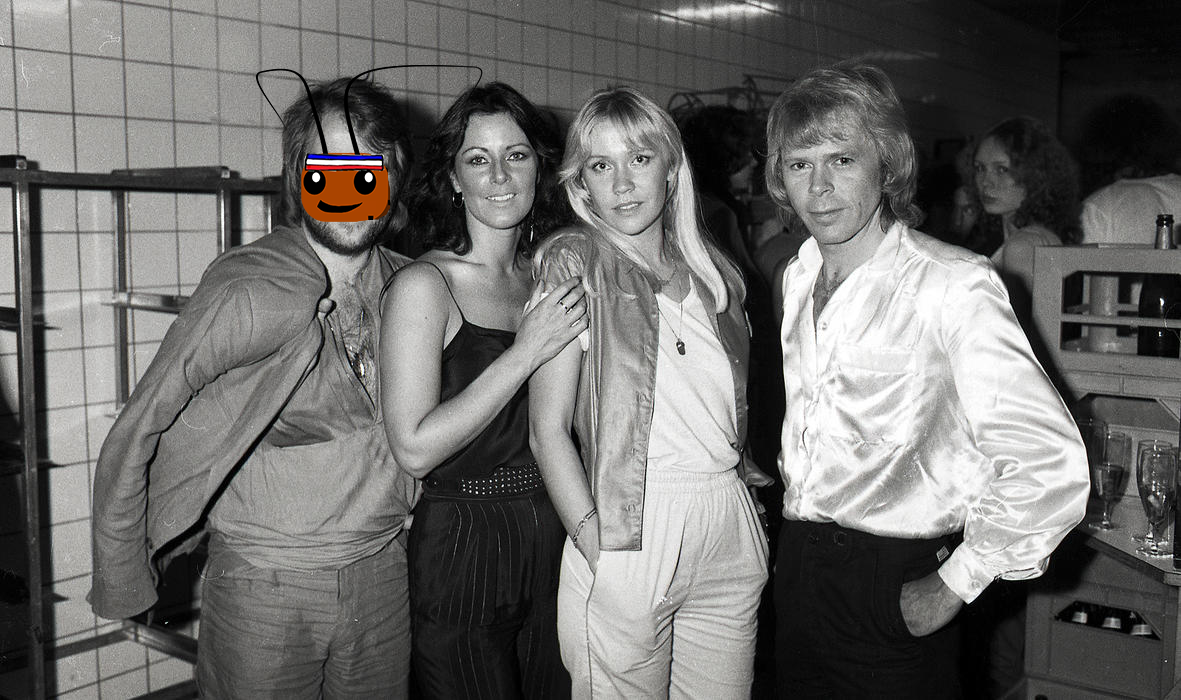
\includegraphics[scale=0.30]{3}}
\end{center}
\begin{flushleft}
\makebox[\textwidth]{naam:\enspace\hrulefill}
\end{flushleft} }
\question[1] {
\begin{center}
{
\includegraphics[scale=0.15]{4}}
\end{center}
\begin{flushleft}
\makebox[\textwidth]{naam:\enspace\hrulefill}
\end{flushleft} }
\question[1] {
\begin{center}
{
\includegraphics[scale=0.80]{5}}
\end{center}
\begin{flushleft}
\makebox[\textwidth]{naam:\enspace\hrulefill}
\end{flushleft} }

\question[3]{
{
\begin{table}[h]
\centering
\begin{tabular}{llll}
\textbf{Amerikaan} & \textbf{Verbranding}          & \textbf{Rapper} & \textbf{Nummer}    \\
\textbf{Zweepslag}      & \textbf{Van voor naar achter} & \textbf{Acteur}       & \textbf{Genie in Aladdin }   \\
\textbf{Auschwitz} & \textbf{Letsel}           & \textbf{Joden}          & \textbf{Nek}
\end{tabular}
\end{table}
}
\begin{flushleft}
\makebox[\textwidth]{Link 1:\enspace\hrulefill\linebreak}
\makebox[\textwidth]{Link 2:\enspace\hrulefill}
\makebox[\textwidth]{Link 3:\enspace\hrulefill}
\end{flushleft}
}

\question[3]{
{\begin{table}[h]
\centering
\begin{tabular}{llll}
\textbf{VTM} & \textbf{Citroen}          & \textbf{Brussel} & \textbf{Sunrise}    \\
\textbf{CSI}      & \textbf{Parijs} & \textbf{Mexicaans}       & \textbf{The Simpsons}   \\
\textbf{London} & \textbf{Zout}           & \textbf{Amsterdam}          & \textbf{Temptation Island }
\end{tabular}
\end{table}
}
\begin{flushleft}
\makebox[\textwidth]{Link 1:\enspace\hrulefill}
\makebox[\textwidth]{Link 2:\enspace\hrulefill}
\makebox[\textwidth]{Link 3:\enspace\hrulefill}
\end{flushleft}
}

\question[3]{
{\begin{table}[h]
\centering
\begin{tabular}{llll}
\textbf{Bieten} & \textbf{Klein}          & \textbf{De pil} & \textbf{Condoom}    \\
\textbf{Kristalstructuur}      & \textbf{Spielberg} & \textbf{Pessarium}       & \textbf{Telefoneren}   \\
\textbf{Riet} & \textbf{Buitenaards}           & \textbf{CH20}          & \textbf{Spiraaltje}
\end{tabular}
\end{table}
}
\begin{flushleft}
\makebox[\textwidth]{Link 1:\enspace\hrulefill}
\makebox[\textwidth]{Link 2:\enspace\hrulefill}
\makebox[\textwidth]{Link 3:\enspace\hrulefill}
\end{flushleft}
}
\newpage
\question[3]{
{\begin{table}[h]
\centering
\begin{tabular}{llll}
\textbf{Dagboek} & \textbf{Papier}          & \textbf{Joods meisje} & \textbf{Bezem}    \\
\textbf{Onderduiken}      & \textbf{Kraanvogel} & \textbf{Brandstapel}       & \textbf{Japans}   \\
\textbf{Vouwen} & \textbf{vrouw}           & \textbf{Schuilhuis}          & \textbf{Neuswrat}
\end{tabular}
\end{table}
}
\begin{flushleft}
\makebox[\textwidth]{Link 1:\enspace\hrulefill}
\makebox[\textwidth]{Link 2:\enspace\hrulefill}
\makebox[\textwidth]{Link 3:\enspace\hrulefill}
\end{flushleft}
}
\question[3]{
{\begin{table}[h]
\centering
\begin{tabular}{llll}
\textbf{Neuswrat} & \textbf{rapper}          & \textbf{brandstapel} & \textbf{papier}    \\
\textbf{Amerikaan}      & \textbf{Kraanvogel} & \textbf{bezem}       & \textbf{genie in Alladin}   \\
\textbf{vouwen} & \textbf{vrouw}           & \textbf{Acteur}          & \textbf{Japans}
\end{tabular}
\end{table}
}
\begin{flushleft}
\makebox[\textwidth]{Link 1:\enspace\hrulefill}
\makebox[\textwidth]{Link 2:\enspace\hrulefill}
\makebox[\textwidth]{Link 3:\enspace\hrulefill}
\end{flushleft}
}

\end{questions}

\begin{table}[!b]
\centering
\begin{tabular}{|l|l|l|l|l|l|l|l|l|l|l|l}
\hline
Vraag       & 1 & 2 & 3 & 4 & 5 & 6 & 7 & 8 & 9 & 10 \\ \hline
max. punten & 1 & 1 & 1 & 1 & 1 & 3 & 3 & 3 & 3 & 3\\ \hline
score       &   &   &   &   &   &   &   &   &   &  \\ \hline
\end{tabular}
\end{table}
\newpage
%
\section{Tafel ronde 2: Wie is het?}
Freddy heeft een paar mooie foto's gevonden van het home Astrid presidium. Kan jij raden wie het is?

Enkel voornaam, fonentisch geschreven
\begin{questions}
\question[1] {
\begin{center}
{\includegraphics[scale=0.20]{robbe}}
\end{center}
\begin{flushleft}
\makebox[\textwidth]{naam:\enspace\hrulefill}
\end{flushleft} }
\question[1] {
\begin{center}
{\includegraphics[scale=0.08]{lisa}}
\end{center}
\begin{flushleft}
\makebox[\textwidth]{naam:\enspace\hrulefill}
\end{flushleft} }
\question[1] {
\begin{center}
{\includegraphics[scale=0.20]{arend}}
\end{center}
\begin{flushleft}
\makebox[\textwidth]{naam:\enspace\hrulefill}
\end{flushleft} }
\question[1] {
\begin{center}
{\includegraphics[scale=0.10]{bart}}
\end{center}
\begin{flushleft}
\makebox[\textwidth]{naam:\enspace\hrulefill}
\end{flushleft} }
\question[1] {
\begin{center}
{\includegraphics[scale=0.20]{michelle}}
\end{center}
\begin{flushleft}
\makebox[\textwidth]{naam:\enspace\hrulefill}
\end{flushleft} }
\question[1] {
\begin{center}
{\includegraphics[scale=0.40]{lemmy}}
\end{center}
\begin{flushleft}
\makebox[\textwidth]{naam:\enspace\hrulefill}
\end{flushleft} }
\question[1] {
\begin{center}
{\includegraphics[scale=0.40]{tibo}}
\end{center}
\begin{flushleft}
\makebox[\textwidth]{naam:\enspace\hrulefill}
\end{flushleft} }
\question[1] {
\begin{center}
{\includegraphics[scale=0.10]{wouter}}
\end{center}
\begin{flushleft}
\makebox[\textwidth]{naam:\enspace\hrulefill}
\end{flushleft} }
\question[1] {
\begin{center}
{\includegraphics[scale=0.40]{elien}}
\end{center}
\begin{flushleft}
\makebox[\textwidth]{naam:\enspace\hrulefill}
\end{flushleft} }
\question[1] {
\begin{center}
{\includegraphics[scale=0.10]{sander}}
\end{center}
\begin{flushleft}
\makebox[\textwidth]{naam:\enspace\hrulefill}
\end{flushleft} }

\end{questions}

\begin{table}[!b]
\centering
\begin{tabular}{|l|l|l|l|l|l|l|l|l|l|l|l}
\hline
Vraag       & 1 & 2 & 3 & 4 & 5 & 6 & 7 & 8 & 9 & 10 \\ \hline
max. punten & 1 & 1 & 1 & 1 & 1 & 1 & 1 & 1 & 1 & 1 \\ \hline
score       &   &   &   &   &   &   &   &   &   &   \\ \hline
\end{tabular}
\end{table}
\newpage
%\section{Tafel ronde 3: raadsel ronde}
\begin{questions}
\question[4] {\begin{flushleft}
{\large Raadsel 1: Twenty-one}
\end{flushleft}
\begin{flushleft}
Dit raadsel komt van de thuisstad van Tibo (cultuur home Astrid). In Koksijde staan er veel wetgevingen op hoogte bouw, dus is er maar één echt super hoog gebouw: de Twenty-one. Rara-ra, het gebouw heeft 21 verdiepen. Nu woont de beste vriend van Freddy op de 21ste verdieping. Elke dag als het mooi weer is neemt hij de lift naar beneden en de trap naar boven. Echter wanneer het slecht weer is neemt hij de lift naar beneden en ook de lift naar boven.
\linebreak
De vraag is, hoe komt dit? Waarom neemt hij niet altijd de lift?
\linebreak
\end{flushleft}
}
\it Hint: op slechte dagen neemt hij een paraplu mee!
\fillwithlines{\stretch{1}}
%raadsel 2
\question[2]{\begin{flushleft}
{\large Raadsel 2: Vogel}
\end{flushleft} Maak een vogel door 2 rechte strepen te plaatsen.\center
\includegraphics[scale=1]{kip}}
\newpage
\question[2]{\begin{flushleft}
{\large Raadsel 3: converteer het symbool naar een decimaal getal.}
\end{flushleft}
\begin{center}
\includegraphics[scale=0.4]{76}
\end{center}
\fillwithlines{2em}
}


\question[2] {\begin{flushleft}
{\large Raadsel 4: Ontcijfer}
\end{flushleft}
\begin{flushleft}
Ontcijfer deze boodschap!
\end{flushleft}
\begin{center}
Oleacahoydnebp xef 4
\end{center}
\it Hint! Kijk naar het nummer van het raadsel!
\fillwithlines{3em}
}

\newpage
\question[2] {\begin{flushleft}
{\large Raadsel 4: Symbolen}
\end{flushleft}
Bepaal de volgende symbolen (mintens 2 aanvullen ,maar maximum 5).
\center
\includegraphics[scale=1]{symbolen}
}



\question[2]{\begin{flushleft}
{\large Raadsel 6: Freddy probeert 8 konoginnnen op een schaakbord te zetten, zonder dat ze elkaar in de weg staan. Een koningin kan elke kant uit, dus ze kan horizontaal, verticaal en diagonaal bewegen. }
\end{flushleft}
\begin{center}

\includegraphics[scale=0.03]{schaakbord2}
\end{center}
\newpage
\question[4]{
Er zijn 4 verschillende dozen gegeven, telkens met bijhorend opschrift:

\vspace{0.2cm}

Doos A: \framebox[0.4\textwidth][l]{Het punt zit niet in doos B}

\vspace{0.2cm}

Doos B: \framebox[0.4\textwidth][l]{Het punt zit niet in doos C}

\vspace{0.2cm}

Doos C: \framebox[0.4\textwidth][l]{Het punt zit in doos D}

\vspace{0.2cm}

Doos D: \framebox[0.4\textwidth][l]{Het punt zit in doos A}
\vspace{0.2cm}

Er is maar één doos die de waarheid spreekt.
Je mag maar 1 doos kiezen en openen! 

\textbf{Er is een wiskundige manier voor deze vraag! men kan dit formaliseren met proposities en eventueel verzamelingenleer.}

{\em Opmerking:} om alle punten te krijgen moet je ook proposities geven!}
}
\newpage
\question[2]{
Er rijd een zwarte auto op een zwarte baan, de gebouwen zijn zwart en de bewoners hebben hun zwarte gordijnen gesloten. De autolichten en straatverlichting zijn gedooft. De auto stopt en laat de zwarte kat oversteken. Hoe komt het dat de autobestuurder de zwarte kat zag?

\fillwithlines{\stretch{1}}
}
\end{questions}
\begin{table}[!b]
\centering
\begin{tabular}{|l|l|l|l|l|l|l|l|l|l|l|}
\hline
Vraag       & 1 & 2 & 3 & 4 & 5 & 6 & 7 & 8 \\ \hline
max. punten & 4 & 2 & 2 & 2 & 2 & 2 & 4 & 2 \\ \hline
score       &   &   &   &   &   &   &   &   \\ \hline
\end{tabular}
\end{table}

\end{document}